\chapter{Firegex}

Firegex è un firewall innovativo e multifunzionale, ideato per essere avviato con 0 configurazioni in modo rapido e semplice, agendo principalmente a
livello applicativo di modo da permettere un'analisi del traffico specifica e dettagliata per ogni servizio.
Esistono al suo interno diversi moduli che permettono la creazione di filtri di diversa natura, in modo semplice, flessibile e quanto meno invasivo ed impattante sulle prestazioni della macchina,
mantenendo sempre la massima priorità sulla disponibilità e la corretta funzionalità del servizio stesso.
Il contesto per cui è stato pensato è quello delle competizioni CTF di tipo Attack/Defense, dove vi sono particolari esigenze (descritte nel capitolo precedente),
che Firegex cerca di soddisfare, semplificandone il suo utilizzo, e soprattutto fornendo soluzioni flessibili e adattabili ai requisiti spesso fortemente dinamici dei servizi.

\begin{figure}[H]
    \centering
    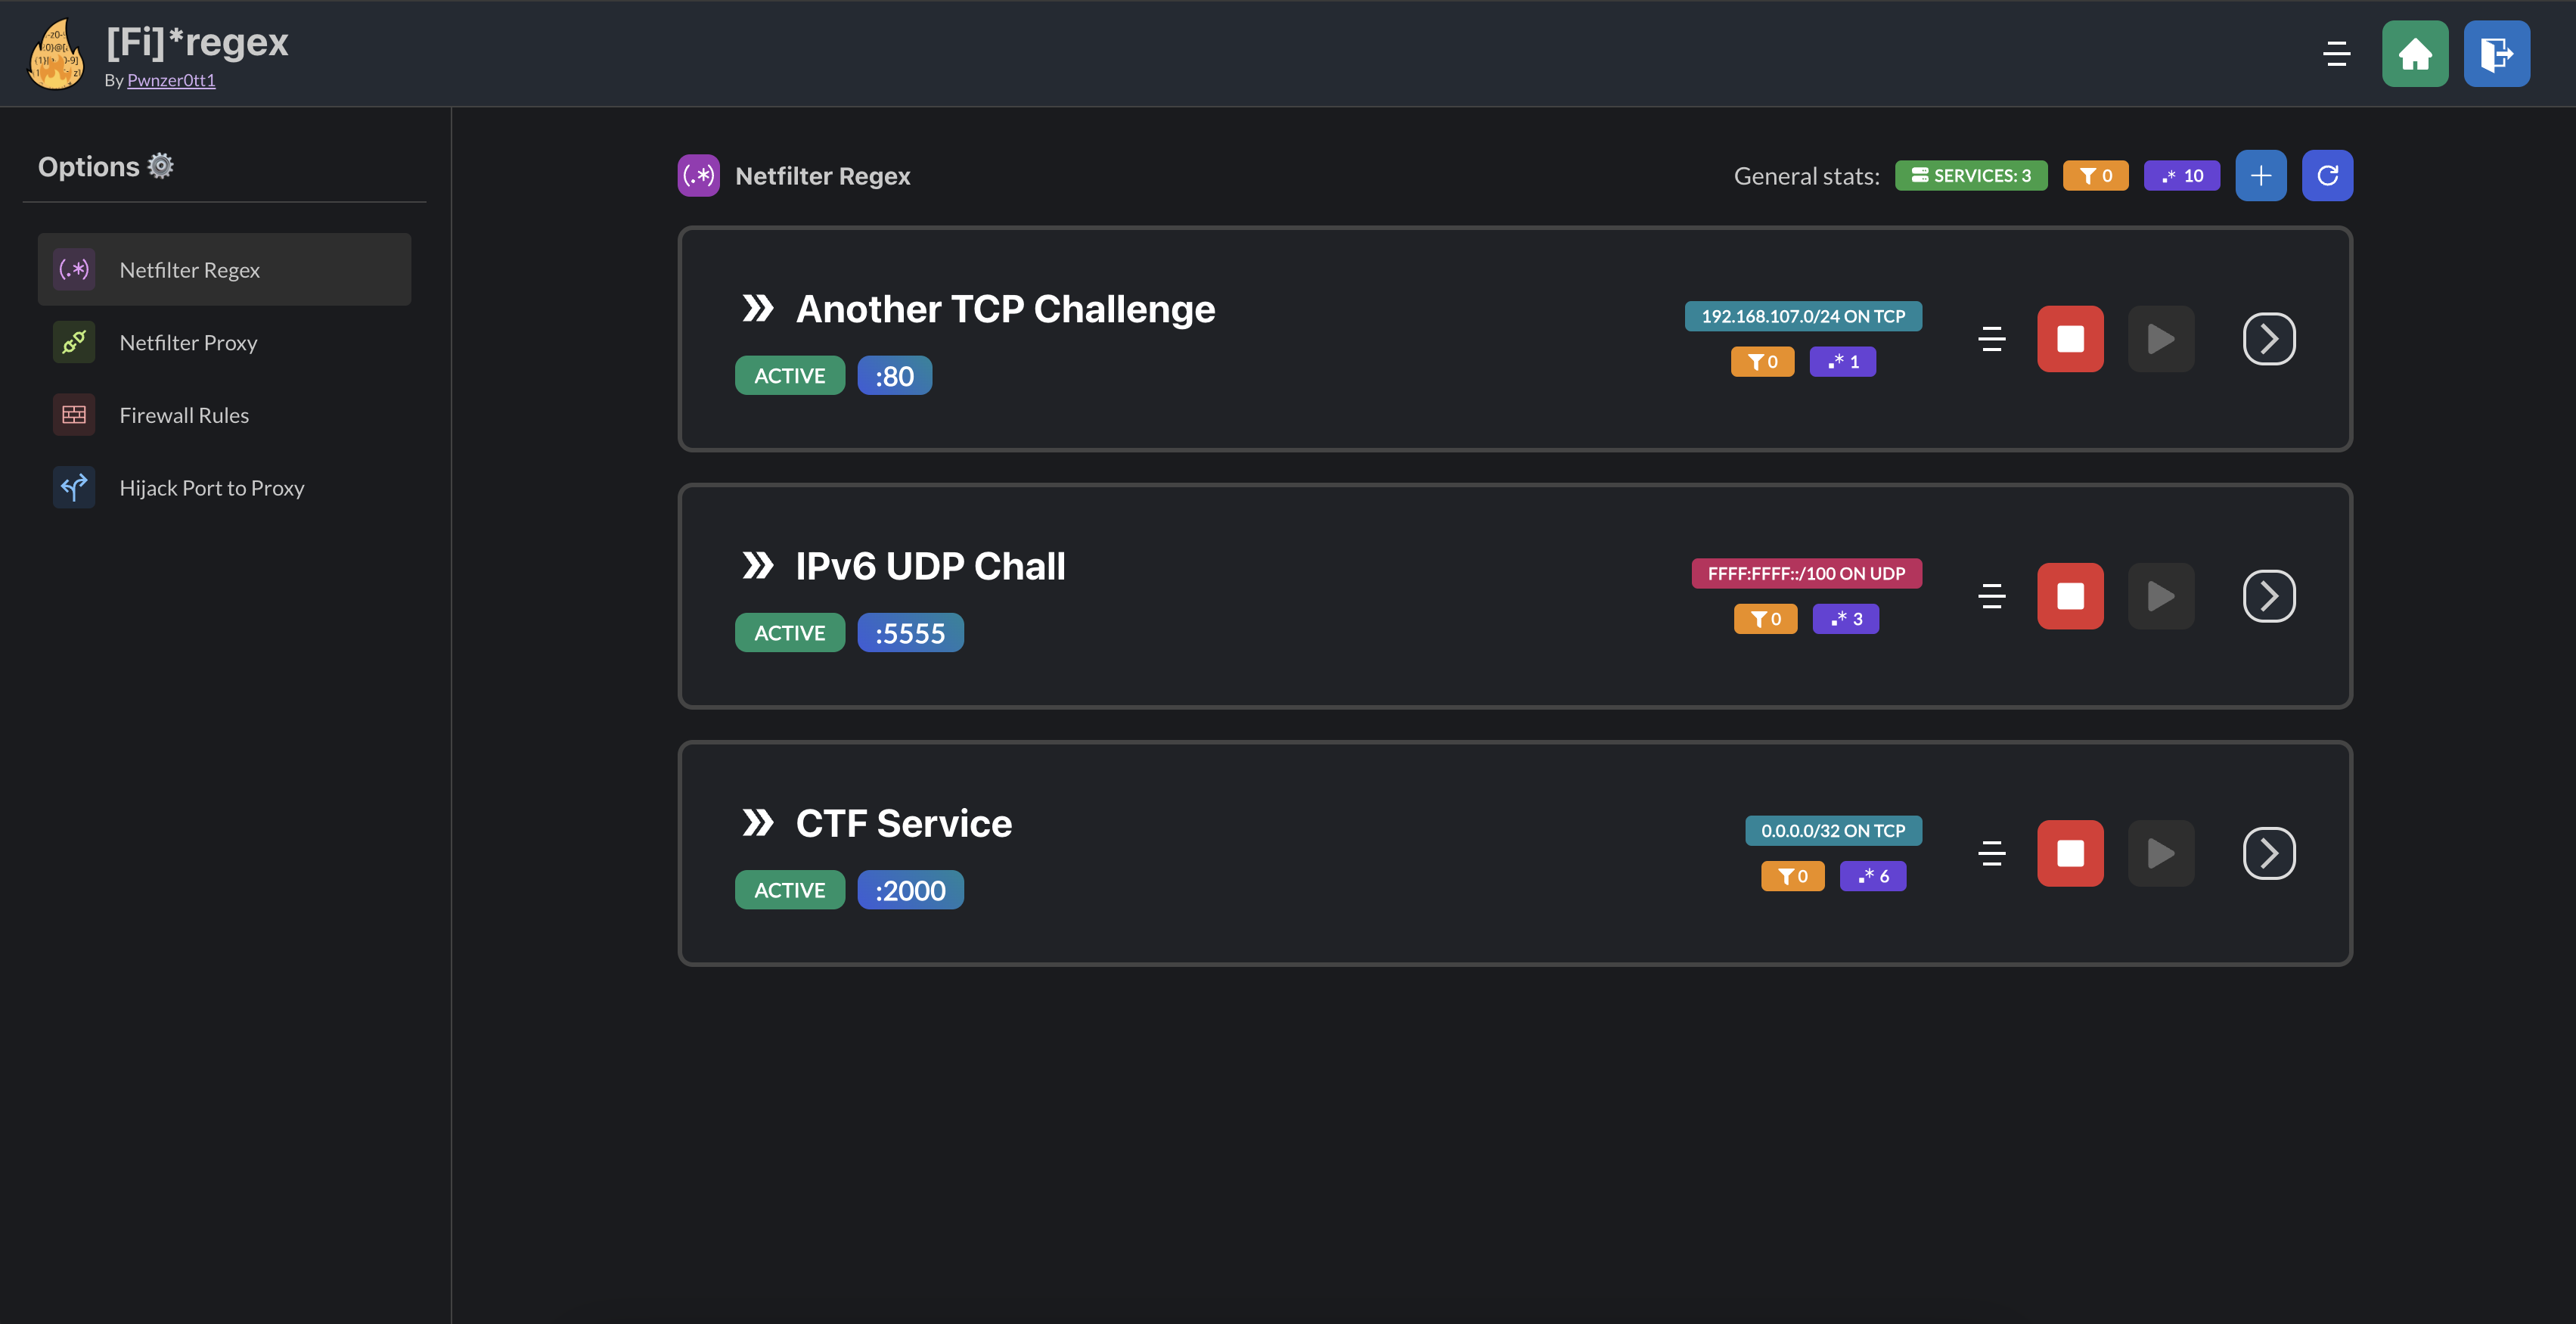
\includegraphics[width=1\textwidth]{images/chapter2/Firegex_Screenshot.png}
    \caption{Interfaccia grafica di Firegex}\label{fig:firegex_frontend}
\end{figure}

\section{Perché nasce Firegex?}

Firegex (come detto in precedenza) nasce dal gruppo che ha affrontato la gara nazionale di Cyberchallenge\footcite{\url{https://cyberchallenge.it/}}{cyberchallenge}
del 2022 al Politecnico di Bari\footcite{\url{https://www.poliba.it}}{poliba_website}, come un normale proxy con filtri basati sulle regex, che col tempo si è evoluto aggiungendo nuove
funzionalità sempre più efficienti, sicure e funzionali alla competizione stessa.\\
La necessità dello sviluppo è nata proprio dalla mancanza di un sistema di difesa che fosse immediato da utilizzare, che non richiedesse configurazioni complesse per
essere avviato, e che permettesse in maniera semplice di costruire dei filtri prontamente attivi, funzionanti e stabili.\\
Durante il suo sviluppo firegex si è sempre più focalizzato su alcuni punti chiave che lo rendono unico rispetto ad altre soluzioni presenti:

\begin{itemize}
    \item \textbf{Trasparenza totale:} La creazione di un proxy comporta una serie di cambiamenti sulla configurazione delle porte di rete esposte dai servizi, l'avvio e la gestione del processo del proxy stesso, e utilizzo di meccanismi di fallback per ovviare ad eventuali problematiche. Queste complicanze erano solo parzialmente gestite inizialmente da firegex, ma con le nuove implementazioni è possibile applicare regole sul traffico senza cambiamenti nelle configurazione, grazie a particolari funzionalità utilizzate, disponibili nel kernel linux, nascondendone però tutta la complessità gestita internamente per il loro corretto funzionamento.
    \item \textbf{Integrazione di tecnologie multiple:} Come già detto, Firegex utilizzava come unico meccanismo di filtraggio le regex, che venivano applicate sui pacchetti di rete per individuare eventuali attacchi. Negli anni si è notato come questo approccio spesso potesse essere limitante, per cui sono stati implementati nuovi meccanismi e tecnologie di filtraggio aumentando la precisione con cui è possibile analizzare il traffico. La seguente tesi tratterà dello sviluppo di una nuova funzionalità particolarmente flessibile denominata \texttt{nfproxy}.
    \item \textbf{Affidabilità e disponibilità:} In ambienti dove la continuità del servizio è critica, è fondamentale che il sistema di sicurezza non diventi un collo di bottiglia. Firegex è stato progettato per garantire un’elevata disponibilità, avendo meccanismi di fallback applicati in caso di errori critici, e offrendo soluzioni rapide per il ripristino della configurazione in caso di errori e per il reset immediato dei filtri applicati.
    \item \textbf{Facilità di utilizzo:} Nelle A/D il tempo è una risorsa fondamentale: gli strumenti a disposizione per la gara non devono richiedere eccessivi tempi di configurazione, che tendenzialmente andrebbe automizzata, e facilitare la risoluzione di problemi semplificando eventuali fasi di troubleshooting, che possibilmente andrebbero evitate. L'obiettivo infatti è quello di focalizzare l'attenzione sull'individuazione di vulnerabilità, che rappresenta un necessità chiave nella competizione. Firegex è stato progettato per essere quanto meno dispersivo possibile, avere configurazioni semplici e guidate, un'interfaccia intuitiva, e gestire autonomamente tutte le problematiche legate alla gestione dei filtri e alla loro gestione ed esecuzione.
\end{itemize}

\section{Confronto con altre soluzioni}

Firegex si distingue rispetto ad altre soluzioni presenti, come \texttt{CTF proxy}\footcite{\url{https://github.com/ByteLeMani/ctf_proxy}}{ctf_proxy}, \texttt{Nginx}\footcite{\url{https://nginx.org/}}{nginx}, \texttt{Suricata}\footcite{\url{https://suricata.io/}}{suricata} o \texttt{Fortinet}\footcite{\url{https://www.fortinet.com/}}{fortinet} per diverse motivazioni:\\

\renewcommand{\arraystretch}{2}
\begin{table}[H]
    \centering
    \setlength{\tabcolsep}{12pt}
    \begin{tabular}{|c|c|c|c|c|}
        \hline
        \begin{tabular}[c]{@{}c@{}} \textbf{Firewall} \end{tabular} & 
        \begin{tabular}[c]{@{}c@{}} \textbf{0 Config Run}  \end{tabular} & 
        \begin{tabular}[c]{@{}c@{}} \textbf{Easy use} \end{tabular} & 
        \begin{tabular}[c]{@{}c@{}} \textbf{Easy Filter Add} \end{tabular} & 
        \begin{tabular}[c]{@{}c@{}} \textbf{Flexible} \end{tabular} \\
        \hline
        \texttt{Firegex} & 
        \begin{tabular}[c]{@{}c@{}} \color{Green}\faIcon[solid]{check-circle} \end{tabular} & 
        \begin{tabular}[c]{@{}c@{}} \color{Green}\faIcon[solid]{check-circle} \end{tabular} & 
        \begin{tabular}[c]{@{}c@{}} \color{Green}\faIcon[solid]{check-circle} \end{tabular} & 
        \begin{tabular}[c]{@{}c@{}} \color{Green}\faIcon[solid]{check-circle} \end{tabular} \\
        \hline
        \texttt{Nginx} & 
        \begin{tabular}[c]{@{}c@{}} \color{Orange}\faIcon[solid]{exclamation-circle} \end{tabular} & 
        \begin{tabular}[c]{@{}c@{}} \color{Orange}\faIcon[solid]{exclamation-circle} \end{tabular} & 
        \begin{tabular}[c]{@{}c@{}} \color{Orange}\faIcon[solid]{exclamation-circle} \end{tabular} & 
        \begin{tabular}[c]{@{}c@{}} \color{Orange}\faIcon[solid]{exclamation-circle} \end{tabular} \\
        \hline
        \texttt{CTF proxy} & 
        \begin{tabular}[c]{@{}c@{}} \color{Red}\faIcon[solid]{times-circle} \end{tabular} & 
        \begin{tabular}[c]{@{}c@{}} \color{Orange}\faIcon[solid]{exclamation-circle} \end{tabular} & 
        \begin{tabular}[c]{@{}c@{}} \color{Orange}\faIcon[solid]{exclamation-circle} \end{tabular} & 
        \begin{tabular}[c]{@{}c@{}} \color{Green}\faIcon[solid]{check-circle} \end{tabular} \\
        \hline
        \texttt{Fortinet} & 
        \begin{tabular}[c]{@{}c@{}} \color{Red}\faIcon[solid]{times-circle} \end{tabular} & 
        \begin{tabular}[c]{@{}c@{}} \color{Red}\faIcon[solid]{times-circle} \end{tabular} & 
        \begin{tabular}[c]{@{}c@{}} \color{Orange}\faIcon[solid]{exclamation-circle} \end{tabular} & 
        \begin{tabular}[c]{@{}c@{}} \color{Orange}\faIcon[solid]{exclamation-circle} \end{tabular} \\ 
        \hline
        \texttt{Suricata} & 
        \begin{tabular}[c]{@{}c@{}} \color{Red}\faIcon[solid]{times-circle} \end{tabular} & 
        \begin{tabular}[c]{@{}c@{}} \color{Orange}\faIcon[solid]{exclamation-circle} \end{tabular} & 
        \begin{tabular}[c]{@{}c@{}} \color{Orange}\faIcon[solid]{exclamation-circle} \end{tabular} & 
        \begin{tabular}[c]{@{}c@{}} \color{Orange}\faIcon[solid]{exclamation-circle} \end{tabular} \\
        \hline
    \end{tabular}
    \caption{Confronto tra le soluzioni per il firewall}\label{tab:firewall_compare}
\end{table}
\renewcommand{\arraystretch}{1}

\begin{itemize}
    \setlength{\itemsep}{2pt}
    \setlength{\parskip}{2pt}
    \item \textbf{Nginx} è una soluzione molto flessibile ed affidabile, ma richiede configurazioni complesse e non permette di applicare filtri in maniera immediata e trasparente, ha necessità di cambiare porte e non supporta nativamente filtri più avanzati come quello trattato in questa tesi. Non ha una interfaccia grafica per la gestione delle regole.
    \item \textbf{CTF proxy} è una soluzione fortemente flessibile ed affidabile, ma richiede la creazione di configurazioni e allo stesso modo necessita di cambiare porte ai servizi originali, inoltre a suo supporto non esiste un'interfaccia semplice da usare.
    \item \textbf{Fortinet} è una soluzione estremamente affidabile, ben riconosciuta nel settore, ma richiede configurazioni complesse ed è per questo molto lento da avviare. Il suo operato inoltre potrebbe causare diversi problemi, essendo molto invasivo nel sistema. Il suo utilizzo è poco pratico per l'utilizzo in competizioni CTF, nonostante rappresenti una delle principali soluzioni fuori da questo contesto.\@
    \item \textbf{Suricata} è una soluzione molto affidabile che offre un grado di flessibilità intermedio, ma pecca della mancanza di un'interfaccia semplice per il suo utilizzo, e richiede configurazioni per essere avviato.
\end{itemize}
\newpage
\section{Architettura}

Firegex, avendo un interfaccia web, è composto da un frontend scritto in \texttt{react}\footcite{\url{https://react.dev/}}{react} e un backend sviluppato con \texttt{fastapi}\footcite{\url{https://fastapi.tiangolo.com/}}{fastapi}. Il backend utilizza inoltre dei moduli scritti in C++ per le funzionalità più critiche, come per lo scambio dei pacchetti lato kernel e l'elaborazione in tempo reale delle espressioni regolari. Inoltre per funzionare, fa intenso utilizzo delle funzionalità di \texttt{nftables}\footcite{\url{https://netfilter.org/projects/nftables/}}{nftables}, e di \texttt{netfilter\_queue}\footcite{\url{https://netfilter.org/projects/libnetfilter_queue/}}{netfilter_queue} (brevemente \texttt{nfqueue}). L'intera infrastruttura è avviata tramite \texttt{docker}\footcite{\url{https://www.docker.com/}}{docker} che ne permette un avvio con 0 configurazioni e immediato: \texttt{docker} è usualmente lo strumento principale per l'avvio di servizi in competizioni CTF, pertanto nella maggior parte dei casi è già presente e configurato correttamente.

\begin{figure}[H]
    \centering
    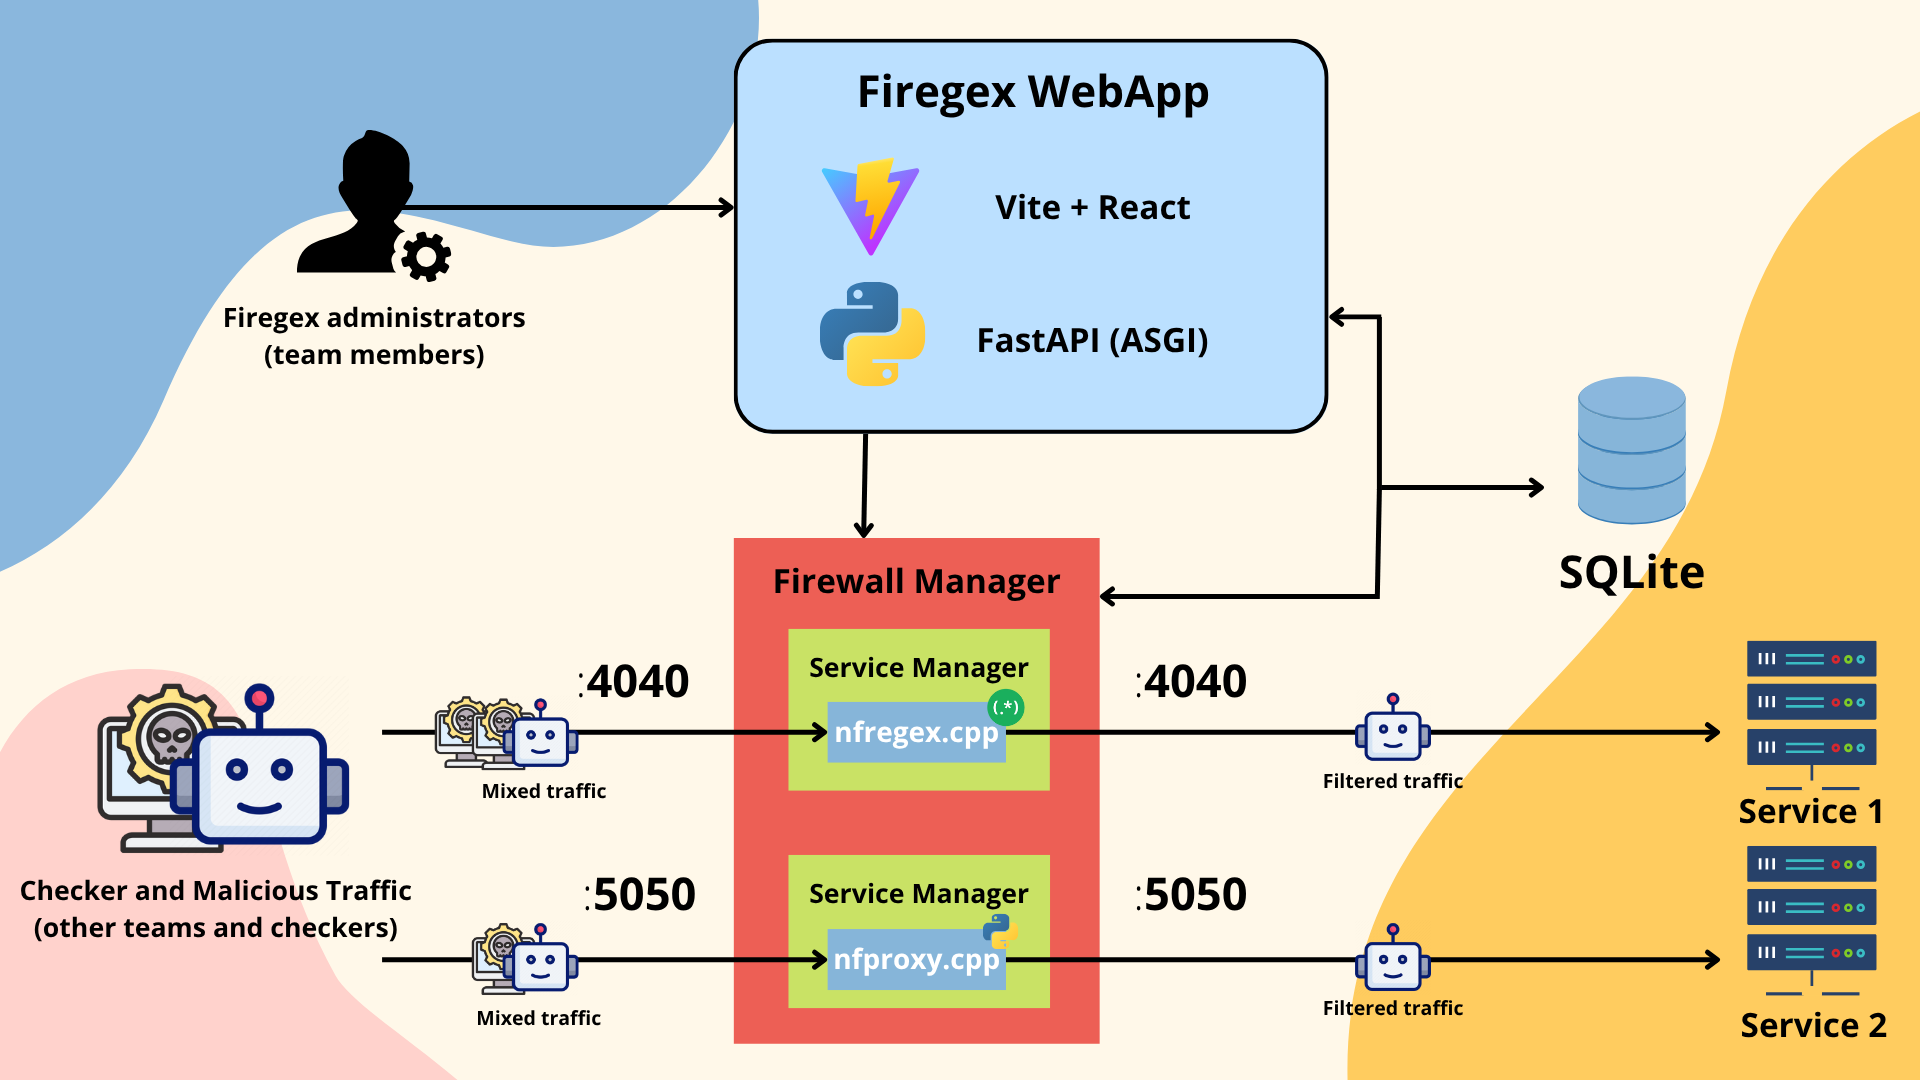
\includegraphics[width=0.98\textwidth]{images/chapter2/FiregexInternals.png}
    \caption{Schema generale dell'architettura di Firegex}\label{fig:firegex_arch}
\end{figure}

\subsection{Frontend e Backend}
\begin{itemize}
    \item \textbf{Frontend (React):} L'interfaccia utente risulta fortemente interattiva e intuitiva nelle fasi di creazione dei filtri, nel loro monitoraggio e la gestione degli stessi. L'interfaccia è parte fondamentale di Firegex, poichè consente di soddisfare uno dei punti chiave del progetto: la semplicità di utilizzo.
    \item \textbf{Backend (FastAPI + C++):} Il backend è realizzato utilizzando FastAPI, un framework moderno e ad alte prestazioni per la creazione di API HTTP, integrato con moduli critici scritti in C++. Questa combinazione consente di gestire le richieste in maniera estremamente veloce ed affidabile, garantendo al contempo, l'esecuzione delle operazioni critiche a livello di rete con le performance di un linguaggio a basso livello. Il backend python tuttavia svolge anche un ruolo attivo nell'applicazione delle regole di rete tramite il modulo ufficiale di \texttt{libnftables}\footcite{\url{https://git.netfilter.org/nftables/tree/py}}{nftables_python}.
\end{itemize}

\subsection{Moduli C++}
Le parti critiche di networking gestite da Firegex sono implementate in C++. Questi moduli sono responsabili del filtraggio diretto scambiando pacchetti con il kernel e implementano la logica di filtraggio per i moduli \texttt{nfregex} e \texttt{nfproxy}, facendo utilizzo di librerie ad altre prestazioni come \texttt{libtins}\footcite{\url{https://libtins.github.io/}}{libtins}, \texttt{libmnl}\footcite{\url{https://netfilter.org/projects/libmnl/}}{libmnl}, \texttt{vectorscan}\footcite{\url{https://vectorcamp.gr/project/vectorscan/}}{vectorscan} (specificatamente per \texttt{nfregex}), e le C API di \texttt{python}\footcite{\url{https://docs.python.org/3/c-api/}}{python_c_api} (specificatamente per \texttt{nfproxy}).

Ciò permette di fornire le seguenti caratteristiche:

\begin{itemize}
    \item \textbf{Prestazioni elevate:} Grazie all'efficienza del linguaggio C++ e alla possibilità di gestire low level le interazione con il sistema operativo, il filtraggio del traffico avviene con latenze estremamente ridotte.
    \item \textbf{Parallelizzazione:} I filtri che richiedono elaborazione userspace facendo uso di nfqueue, sono gestiti in un sistema di elaborazione multi-thread, garantendo una gestione ottimale del traffico in situazioni di carico elevato e con un numero di connessioni elevate.
    \item \textbf{Integrazione con librerie di rete:} L'utilizzo di librerie specializzate come libtins e libmnl consente di implementare funzionalità avanzate mantenendo affidabilità su come vengono elaborati i pacchetti in rete e prestazioni elevate nell'elaborazione.
\end{itemize}

\subsection{Netfilter nftables}

nftables rappresenta il framework moderno per il filtraggio dei pacchetti e la gestione del traffico nelle distribuzioni Linux. In Firegex, nftables viene utilizzato per:
\begin{itemize}
    \item \textbf{Applicare regole di sicurezza:} Le regole di firewall vengono implementate tramite nftables, garantendo un controllo granulare sul traffico di rete.
    \item \textbf{Reindirizzamento del traffico:} La funzionalità \texttt{porthijack} si basa su regole di nftables per deviare il traffico da una porta a un’altra, consentendo l’implementazione di un proxy interno che si occuperà di filtrare e inoltrare il traffico al servizio originale.
    \item \textbf{Integrazione con nfqueue:} nftables lavora in sinergia con il modulo nfqueue per intercettare i pacchetti e inoltrarli allo spazio utente per ulteriori analisi.
\end{itemize}

Le funzionalità precedentemente citate saranno meglio trattate nei paragrafi successivi.

\subsection{Netfilter Queue Module}
Il modulo Netfilter Queue (nfqueue) gioca un ruolo fondamentale nell'architettura di Firegex, consentendo l'intercettazione dei pacchetti direttamente a livello kernel e il loro inoltro allo spazio utente. Le sue principali caratteristiche includono:
\begin{itemize}
    \item \textbf{Intercettazione diretta:} nfqueue permette di catturare il traffico di rete e accodarlo ad una coda, in attesa di essere elaborato da un'applicazione utente: questo permette allo sviluppatore di avere accesso ai pacchetti dal layer di rete, permettendo anche l'analisi e la modifica degli header, normalmente non accessibili tramite un proxy. Inoltre intercettare i pacchetti in questo modo rende l'operazione di filtraggio completamente invisibile per l'applicativo, che non necessiterà di riconfigurazioni.
    \item \textbf{Elaborazione in spazio utente:} Una volta intercettati, i pacchetti vengono inoltrati allo spazio utente dove possono essere analizzati e processati da moduli come \texttt{nfregex} e \texttt{nfproxy}, consentendo l'utilizzo di logiche di filtraggio avanzate ma comunque evitando di portare codice potenzialmente pericoloso lato kernel che potrebbe compromettere la stabilità del sistema.
\end{itemize}

\section{Funzionalità}

All'interno di Firegex sono presenti attualmente 4 moduli principali, ognuno con delle funzionalità specifiche che permettono di applicare filtri con tecnologie e funzionalità differenti. I moduli sono \texttt{nfregex}, \texttt{firewall}, \texttt{porthijack} e \texttt{nfproxy}. All'interno di questi moduli firegex possiede una documentazione interna alla piattaforma stessa che permette di comprendere come utilizzare le funzionalità offerte, e come configurare i filtri in maniera corretta.\\

Firegex è avviabile tramite un unico comando, supponendo che \texttt{docker}\footcite{\url{https://www.docker.com/}}{docker} sia già installato nel sistema:\\
\mintinline{bash}{sh <(curl -sLf https://pwnzer0tt1.it/firegex.sh)}

\subsection{nfregex}
Il modulo \texttt{nfregex} (pensato originariamente come unico e principale) possiede funzionalità per la creazione di filtri basati su espressioni regolari. Utilizzando \texttt{nfqueue} in combinazione con \texttt{nftables}, questo modulo intercetta le richieste di rete direttamente a livello kernel. La funzionalità permette l'utilizzo di regex \texttt{PCRE2}\footcite{\url{https://www.pcre.org/}}{pcre_website} compliant tramite l'utilizzo di \texttt{vectorscan}\footcite{\url{https://vectorcamp.gr/project/vectorscan/}}{vectorscan} (fork di \texttt{hyperscan}\footcite{\url{http://hyperscan.io/}}{hyperscan} compatibile con arm64) per garantire prestazioni elevate e una corretta elaborazione delle regole. La funzionalità supporta IPv4 e IPv6, e protocolli di livello superiore come TCP e UDP.\@ Per i pacchetti TCP, la regex viene applicata all'intero flusso ricostruito e ordinato, tramite le \texttt{stream regex} disponibili in vectorscan.

\subsection{firewall}
La funzionalità \texttt{firewall} di Firegex offre un controllo completo sul traffico di rete, tramite regole simili a quelle offerte da strumenti tradizionali come \texttt{ufw} o \texttt{iptables}. Dispone quindi di funzionalità basilari e potrebbe risultare utile per applicare questa tipologia di regole evitando l'utilizzo di ulteriori tool di filtering che potrebbero entrare in conflitto con firegex.

\subsection{porthijack}
Il modulo \texttt{porthijack} introduce la capacità di reindirizzare il traffico destinato ad una determinata porta verso un’altra. Questa funzionalità è particolarmente utile in scenari dove si ha il bisogno di costruire un proxy personalizzato, ma si vuole evitare la riconfigurazione del servizio di base. Port hijacking infatti consente di impostare un redirect del traffico dall'interfaccia su cui il servizio viene esposto nella rete di gara, dirottandolo per un proxy in localhost, che poi tramite la stessa interfaccia di loopback inoltrerà il traffico al servizio originale.

\subsection{nfproxy}
\texttt{nfproxy}, il modulo trattato in questa tesi, sfrutta le funzionalità di \texttt{nfqueue} per l'intercettazione del traffico, simulando lato utilizzatore il comportamento di un tradizionale proxy python. Le caratteristiche principali del modulo sono:
\begin{itemize}
    \setlength{\itemsep}{1pt}
    \setlength{\parskip}{1pt}
    \item \textbf{Sviluppo in Python:} Permette agli sviluppatori di scrivere e integrare filtri personalizzati in linguaggio Python, offrendo un altissimo livello di flessibilità per l'analisi del traffico.
    \item \textbf{Parsing avanzato dei protocolli:} Tramite funzionalità predefinite è possibile eseguire la decodifica di protocolli come HTTP, in modo immediato e già disponibile all'utilizzo, senza che queste funzionalità debbano essere implementate manualmente.
    \item \textbf{Test e validazione:} I filtri possono essere provati in anticipo tramite il comando \texttt{fgex}, rendendo possibile la prova del filtro prima si applicarlo al traffico.
    \item \textbf{Interfaccia grafica:} L'interfaccia di dettaglio del servizio permette di visualizzare in tempo reale i log e le eventuali eccezioni che si verificano durante l'esecuzione del filtro.
\end{itemize}

Il seguente modulo è stato introdotto in vista di scenari complessi dove gli elementi da individuare per il corretto filtraggio non sono facilmente individuabili tramite regex: ad esempio se il payload fraudolento fosse nei cookie JWT sarebbe necessario eseguire il decoding per rilevare l'attacco.\\

\begin{figure}[H]
    \centering
    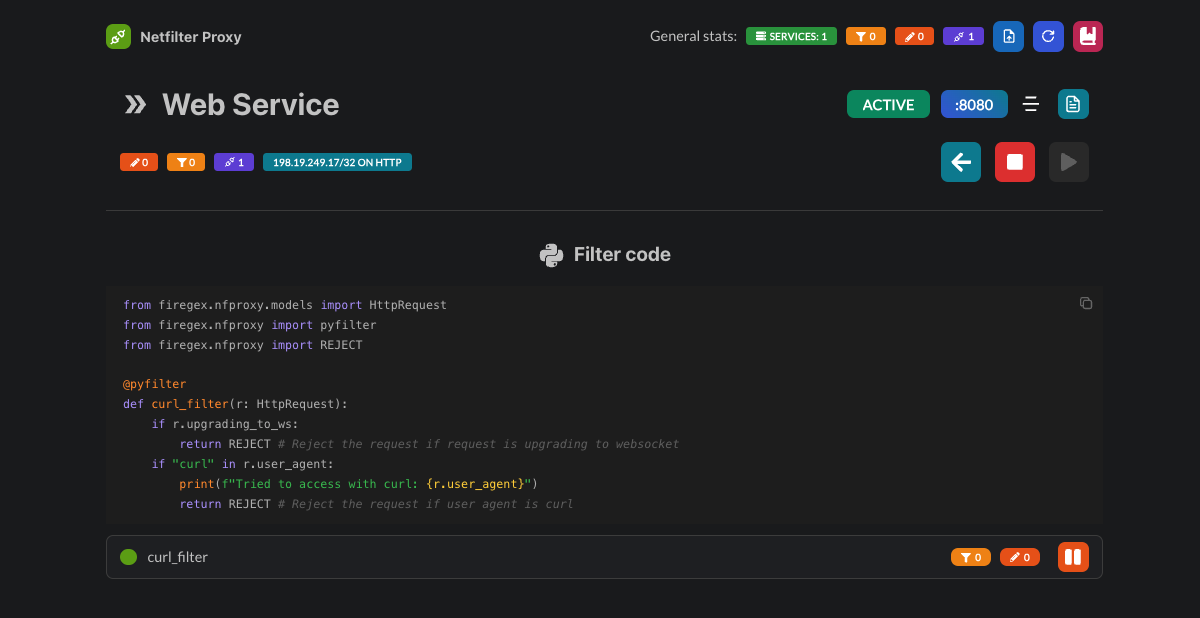
\includegraphics[width=0.83\textwidth]{images/chapter2/NFProxyInterface.png}
    \caption{Interfaccia di dettaglio del servizio nel modulo nfproxy}\label{fig:nfproxy_interface}
\end{figure}

Nei prossimi capitoli verrà trattato in dettaglio lo sviluppo di \texttt{nfproxy}, le sue funzionalità, le problematiche affrontate e le soluzioni adottate.
